\documentclass[11pt,english,a4paper,openright]{report} % Use report because that gives us fancy tables.
\usepackage[english]{babel}
\usepackage[utf8]{inputenc}
\usepackage{amsmath,amsfonts,amsthm,bm} % Math packages 
\usepackage{graphicx} % To include figures
\usepackage{fancyhdr} % Allows for headers
\usepackage{lastpage} % Allows for page numbering in footer
\usepackage{tcolorbox} % To make colourful boxes (objectives)
\usepackage[margin=1.0in]{geometry} % To change page margins
\usepackage[Lenny]{fncychap} % To get fance chapter headings. Options: Sonny, Lenny, Glenn, Conny, Rejne, Bjarne, Bjornstrup
\usepackage{booktabs} % For fancy tables
\usepackage{minted} % To include code in project.
\usepackage{longtable} % For tables spanning multiple pages
\usepackage{hyperref} % To include hyperlinks in the text and footnotes
\usepackage{tikz} % To make cool diagrams
\usetikzlibrary{shapes.geometric, arrows}

\usepackage[style=numeric-comp, sorting=none]{biblatex} % For references, style is to get compressed references [4-12]
\addbibresource{references_books.bib}
\addbibresource{references_tsc.bib}
\addbibresource{references_wind_turbine_monitoring_review.bib}
\addbibresource{references_ml_wind_turbine.bib}
\addbibresource{references_other.bib}

\newcommand{\ra}[1]{\renewcommand{\arraystretch}{#1}} % Something about allowing more space between rows in fancy tables.
\newtheorem{theorem}{Definition} % To allow labelled definitions

\begin{document}

\setlength\parindent{0pt} % Zero Indent in paragraphs

\pagestyle{fancy}

\begin{titlepage}
    \centering
    
    {\LARGE A Literature Review of Time-Series Clustering Techniques and Machine Learning Techniques Used for Monitoring of Wind Turbines} \\ [\baselineskip]
    
    {\Large Written by} \\ 
    {\Large Yohann  Jacob Sandvik } \\

    \begin{abstract}
        This literature review is intended to be a preliminary work for a master thesis. 
        The objectives of the review were to get an overview of machine learning techniques used to monitor wind turbines,
        get an overview of the different feature-based and model-based time-series clustering methods, and determine which
        time-series clustering methods could be relevant for clustering the time series datasets produced by wind turbines in a wind farm.
        96 articles are reviewed for the purpose of fulfilling these objectives. 
        The machine learning methods used for monitoring wind turbines can categorized as regression based models, supervised classification based models
        and unsupervised classification based models. 
        A brief discussion of each category, and the machine learning algorithms within each category is held.
        Many feature-based and model-based representation methods are discussed, as well as many clustering algorithms. 
        The feature-based representation method of principle component analysis (PCA) is tested for exploring a multivariate time series dataset extracted from a wind farm in Norway.
        Finally the different clustering techniques are discussed, and a choice is made as to which representation methods should be further explored in the master thesis: 
        PCA, and autoregressive moving average models.
    \end{abstract}

\end{titlepage}

\pagenumbering{arabic} % Page numbering in the table of contents
\fancyhf{}
%\lhead{left header}
%\rhead{right header}
%\lfoot{left footer}
\rfoot{Page \thepage \hspace{1pt} of \pageref{LastPage}}

\tableofcontents
\newpage
\listoffigures

\listoftables


\chapter{Introduction}

Clustering is a method used to categorize big amounts of data into groups known as \textit{clusters}, when there is little, or no information available about the underlying groups. 
It is a popular choice for extracting patterns from large datasets, because clustering falls within the category of \textit{unsupervised machine learning}, meaning that it does not require the dataset to be labelled. 
Clustering is also a common step in data mining algorithms, where the goal is to learn rules relating the different variables in a dataset. 
In the last decade clustering has started to become more common to use on time-series datasets as they are abundant, and labeling is often costly and time-consuming. 
Time-series clustering has been applied on financial time series, medical time series and time series from a variety of other industries. \bigskip

\section{Motivation}

As of 2018 wind power, together with solar power made up $7\%$ of the world's electricity production,\footnote{\url{https://www.iea.org/geco/electricity/}} and has been referred to as ''the fastest growing source of energy'' by the Norwegian company Statkraft\footnote{\url{https://www.statkraft.com/globalassets/old-contains-the-old-folder-structure/documents/wind-power-aug-2010-eng_tcm9-11473.pdf}}. 
As the effects of climate change steadily are becoming a reality, shifting to renewable energy sources is imperative, and wind power will play a bigger part in meeting the worlds energy demand in the future. \bigskip

To make wind power as a whole more lucrative, a good start would be to reduce the downtime, and improve the performance of turbines. The argument that time-series clustering may be a good approach for this is two-fold. 

\begin{enumerate}
    \item A single wind turbine can have several sensors sampling very often, meaning that a wind farm can produce colossal amounts of time-series data. An unsupervised approach is usefull because labelling of all this data is requires a lot of time and resources.
    \item When wind farms become big enough it will become too costly to manually inspect every turbine to construct an effective model for condition monitoring, further automation is required \cite{espen}. Time-series clustering is therefore a good alternative for condition monitoring.
\end{enumerate}

\section{Objective} \label{sec:objective}

The literature review is meant to be a preliminary work for a master thesis where select techniques will be evaluated on actual time series data produced by a wind farm in Norway. 
To get a better understanding of wind turbines, and the challenges with using machine learning techniques for conddition monitoring of wind turbines, literature on this topic should be reviewed.  
The project assigment is also a continuation of the master thesis written in the spring of 2019 by Espen Waaga. 
In his thesis he explored the effectiveness of clustering raw time series in regards to similarity in time, and shape. 
In his ''Future work'' section Espen Waaga suggests that a natural next step would be to look at clustering with regards to similarity in change, by implementing a model-based approach. 
In addition, due to the quadratic time complexity of the dynamic time warping (DTW) algorithm it is inappropriate to use as a similarity measure for large datasets. 
Therefore, it could be interesting to see if a feature-based approach could be used to cluster time series with regard to similarity in shape with a lower time complexity than the DTW algorithm. 
This literature review has three objectives in the form of questions. \bigskip

\begin{tcolorbox}
    \textbf{Objectives}

    \begin{enumerate}
        \item What machine learning methods are currently being used to monitor the condition, and performance of wind turbines?
        \item What are the different methods of feature-, and model-based time-series clustering currently used?
        \item What time-series clustering methods (if any) are appropriate to test on time-series data produced by wind turbines? 
    \end{enumerate}
\end{tcolorbox}

\section{Structure of Review}

\newpage
\chapter{Method}

\section{Search terms}
To find the relevant literature on the subjects of interest the search engine Oria was used to search the university library of the NTNU. Oria was preferred over other search engines such as Google Scholar because Oria allows one to combine multiple search terms in unison using ''AND'' or ''OR'', and because it allows the user to choose whether the search term should be in the title, subject, or other parts of the articles. The review will only consider articles published in peer-reviewed journals. Table \ref{tab:search_results} summarizes the search results. The \textit{Title} and \textit{General content} columns show which terms were used in the different searches; which terms where required to be in the title, and which terms could be in the ''general content'', meaning any part of the article. Let ''$\times$'' represent the AND operator between two search terms, and ''$\wedge$'' represent the OR operator. The ''*'' operator means that the search will include any word beginning with the word before the star, e.g \textit{detect*} includes \textit{detection}, \textit{detecting}, \textit{detected}, etc. The $N_f$ and $N_i$ columns show how many results each search yielded and how many articles from each search were included in the review, respectively. \bigskip 

\begin{table*}[h]
    \centering
    \ra{1.3}
    \begin{tabular}{ lllrr } 
        \toprule
        Nr. & Title terms & General terms & $N_r$ & $N_i$ \\
        \midrule
        1 & time $\times$ series $\times$ clustering & None & 219 & 121 \\ 
        2 & (monitor* $\wedge{}$ detect*) $\times$ clustering & time $\times$ series & 187 & 21 \\
        3 & wind $\times$ turbine* $\times$ (monitor* $\wedge{}$ detect*) $\times$ review & None & 32 & 3 \\
        4 & wind $\times$ turbine* $\times$ (monitor* $\wedge{}$ detect*) & machine $\times$ learning & 100 & 47 \\ 
        \midrule
        \multicolumn{4}{r}{Total number of articles included} & 193 \\
        \bottomrule
    \end{tabular}
    \caption{Search results}
    \label{tab:search_results}
\end{table*}

\section{Screening method}
To make sure that the articles used were relevant, the review is limited to articles published 2014 or later. Some older articles are included through backward snowballing for their historical importance. There were three levels of screening, screening of the title, abstract, and full article. Title-screening was primarily for seeding out duplicate articles returned from the search-engine. The screening of the abstract and full-article were to identify the articles that were not relevant for the review and exclude them. \bigskip

It has been a challenge to include enough literature to get a good overview of the different methods within time series clustering, but also not more literature the author alone could handle in the time available. So although the objectives is to get an overview of the different time series clustering methods, and an overview of the current machine learning methods used for monitoring wind turbines, the author does not claim to have made a complete exhaustive summary of all the possible methods. \bigskip

When screening articles from search one and two, articles meeting one (or more) of the following criteria were discarded: 
\begin{itemize}
    \item Primary goal is time-series prediction/forecasting. It is outside the scope of this assignment.
    \item Uses subsequence time-series clustering methods. It is outside the scope of this assignment.
    \item Time-series clustering is used only as a minor preprocessing step. Not considered relevant enough to the objectives of the review.
    \item Data used is not time series data. Not considered relevant enough to the objectives of the review.
    \item Paper does not actually use clustering algorithms. Not considered relevant enough to the objectives of the review.
    \item The data used consists of image time series. Data to different from data to be used in master thesis.
    \item The time-series clustering methods explored in the work are \textbf{not} model-based or feature-based. The raw-data-based approach has been somewhat covered in Espen Waaga's master thesis, so work using this appraoch will be emmitted in this review.
\end{itemize}

Search number three was used to find existing literature reviews on condition monitoring of wind turbines. Three good literature reviews on the subject where found, and one good review on machine learning methods used for condition monitoring of wind turbines was found in search four. So, when screening the remaining articles from search number four the focus was to find articles not included in the aforementioned reviews, to complement them as well as possible. \bigskip

\chapter{Wind Turbine Monitoring} \label{s:wt_monitoring}
% First give a short summary of the spectra of different condition monitoring schemes. Importance of predictive maintainance, and \textbf{short summary} of current implementations of predictive maintainance schemes. 

\section{Wind turbine Components}
% Introduce the basic components of a wind turbine, and present some fun statistics about when the different components fail. 
\begin{figure}[h]
    \begin{center}
    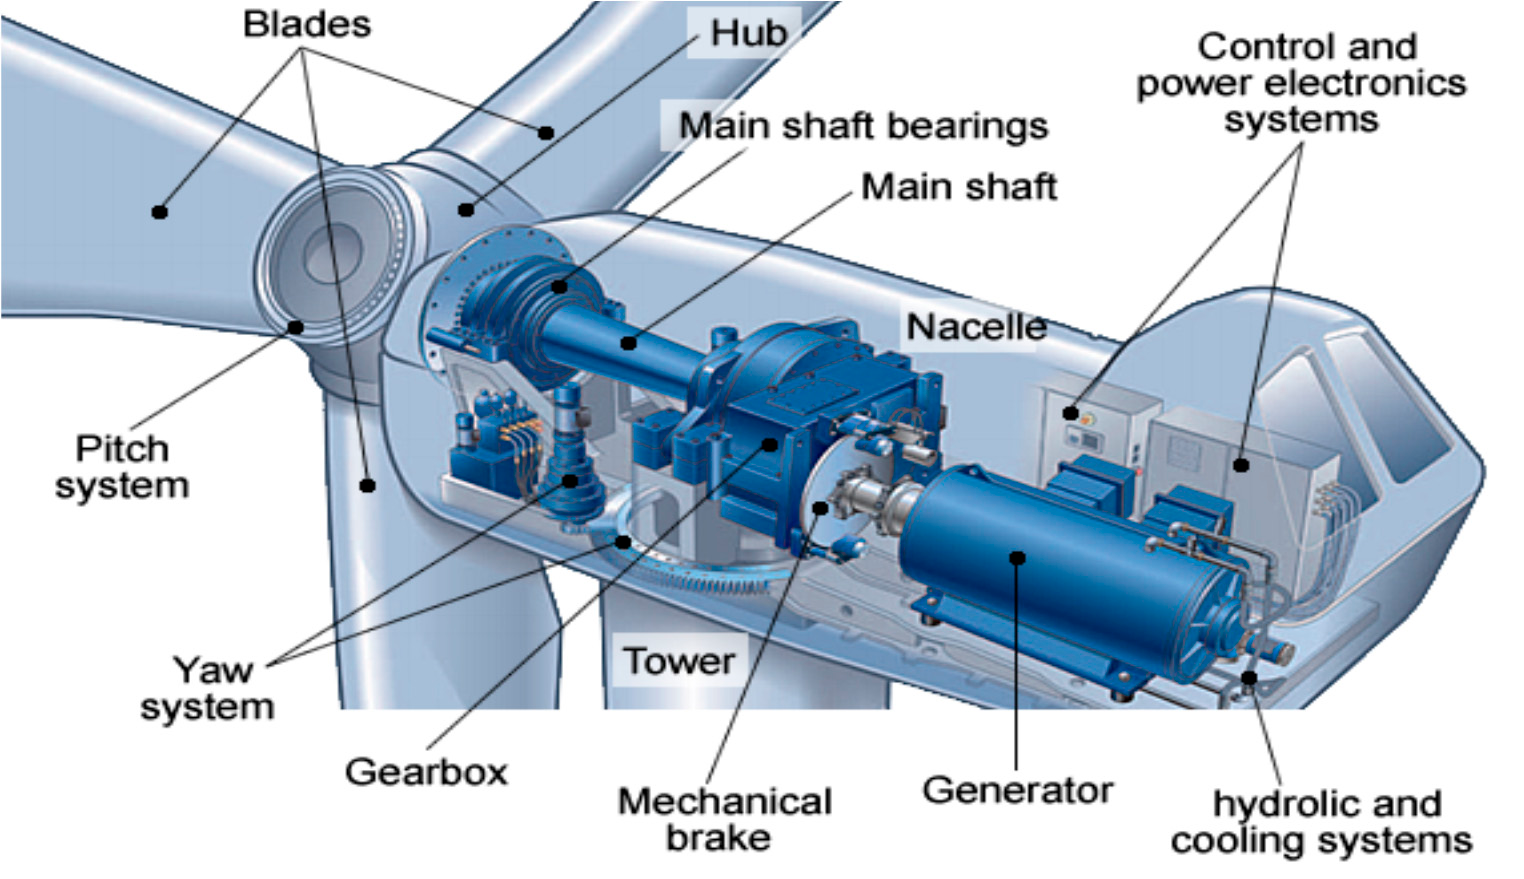
\includegraphics[width=0.8\textwidth]{wind_turbine/wt_parts.png}
    \end{center}
    \caption{Illustration of the different parts of a wind turbine, taken from \cite{adv_meth_for_wt_cond_monit_rev}}
    \label{fig:wt_parts}
\end{figure}

Figure \ref{fig:wt_parts} shows the main parts of a wind turbine which includes the rotor (blades and hub), shafts, gearbox and generator. Simplified a wind turbine works by wind pushing the blades, generating torque that makes the hub rotate. The hub is connected to the gearbox through the main shaft. The gearbox then gears down the torque and gears up the rotational speed to a level that the generator can use to induce current, that goes to a station that transforms the voltage to a level that can be used in the electrical grid. 

\section{Sensors and Data Acquisition}

Information about a wind turbine can come from many sources, it can come from external sources such as images from a camera, or from internal sensors measuring operational data. The collective term for systems measuring operational data is supervisory control and data acquisition (SCADA) systems. To choose what algorithm to use, or what model to use, one must first consider what data one has available. From the literature considered, these where the most used forms of data used as input for the model. 

\begin{itemize}
    \item Vibration measurement  %\cite{wt_bearing_cm_review} \cite{wt_cm_rev_new_trends_chal_2014}
    \item Acustic emission monitoring %\cite{wt_bearing_cm_review} \cite{wt_cm_rev_new_trends_chal_2014}
    \item Temperature measurement %\cite{wt_bearing_cm_review} \cite{wt_cm_rev_new_trends_chal_2014}
    \item Power signal measurement %\cite{wt_bearing_cm_review} \cite{wt_cm_rev_new_trends_chal_2014}
    \item Oil debris monitoring %\cite{wt_bearing_cm_review} \cite{wt_cm_rev_new_trends_chal_2014}
    \item Strain monitoring %\cite{wt_cm_rev_new_trends_chal_2014}
    \item Optical fiber monitoring %\cite{wt_cm_rev_new_trends_chal_2014}
    \item Ultrasonic testing %\cite{wt_cm_rev_new_trends_chal_2014}
    \item Image analysis
\end{itemize}

Analysis of vibration signals is the most common form of condition monitoring used in industry for any form of rotating equipment \cite{wt_bearing_cm_review}. By measuring the acustic emission generated by a component of a wind turbine, one can estimate how much damage it has obtained. The temperature of components in a wind turbine is closely correlated with the health of the component, and is therefore used often in condition monitoring applications \cite{DBN_chicken_swarm_optim}. The power signal can also say a lot about how well a wind turbine is performing, specifically the wind speed - power curve. When monitoring the debris in the oil of a wind turbine gearbox one is analysing the size, type and number of wear particles present in the lubricant, as they can indicate the degree of damage in the gearbox \cite{cm_rnn_lstm}. Strain monitoring, optical fiber monitoring, ultrasonic testing, and image analysis are all used to detect structural damage in different components of the wind turbine, usually the blades \cite{lin_and_non_lin_feat_for_ice_detection_on_blades, image_based_surface_damage_detection_DL_drone_inspection,image_based_YOLO_YSODA, dirt_n_mud_detection_using_guided_waves,blade_defect_detection_imaging_array, unsupervised_AD_blade_damage_deep_features_images}, or tower \cite{wt_cm_rev_new_trends_chal_2014}. The most common approach however was to use a combination of multiple sensors-values to make predictions about the condition about the wind turbine.

\section{Machine learning techniques}
A machine learning is a subset of artificial intelligence. Machine learning models that extract rules from data, which can then be applied to classify, or estimate components of another dataset. Machine learning algorithms are formally divided into \textit{supervised learning}, \textit{unsupervised learning} and \textit{semi-supervised learning}. Supervised learning models require labelled datasets to extract information from the dataset, and are usually used to perform classification tasks, or to estimate a variable that is considered dependent on the input variables (regression). Unsupervised learning algorithms do not require labelled datasets. Semi-supervised learning uses a combination of labelled and unlabelled datasets. \bigskip

\subsection{Feature extraction}
There are two central problems in condition monitoring that can be solved by feature extraction and selection. The first is the sheer volume of information being produced. A wind turbine with only 20 sensors, sampled at 100 Hz will produce 170 MB of information per day. Feature selection is used here to reduce the number of features to only those relevant for condition monitoring. The second problem is that for systems using only one signal such as vibration, there are many components that are superposed to create the measured signal, and noise is present. Feature extraction is used to separate the interesting components from each other, and cancel the noise. For some machine learning models feature extraction is not a neccesary preprocessing step, for others careful though must be given as to how to extract features. Table \ref{tab:feat_ext_wt} shows the most frequent methods found in the articles. 

\begin{table*}
    \centering
    \ra{1.3}
    \begin{tabular}{p{0.31\textwidth}p{0.3\textwidth}}
        \toprule
        Extraction method                   & Articles \\
        \midrule
        ARMA models                         & \cite{ml_cm_wt_blade_ARMA_2018, fault_detection_and_isolation_using_classifier_fusion, lin_and_non_lin_feat_for_ice_detection_on_blades, dirt_n_mud_detection_using_guided_waves, vibration_ARMA_decision_tree_cm_wt} \\
        Discrete Wavelet Transform (DWT)    & \cite{fault_detection_and_isolation_using_classifier_fusion, image_texture_analysis_FD_wt, vibration_acustic_decision_tree_SVM_gearbox, integrated_cm_bearing_fault_wt_gearbox} \\
        Principal Component analysis (PCA)  & \cite{lin_and_non_lin_feat_for_ice_detection_on_blades, multiway_PCA_multivar_inference_cm_wt, dirt_n_mud_detection_using_guided_waves, integrated_cm_bearing_fault_wt_gearbox, unsupervised_AD_blade_damage_deep_features_images, online_fd_using_PCA_different_operating_zones, fault_detect_PARAFAC_k_means}\\
        Basic signal statistics             & \cite{blade_damage_detection_sup_ml_alg, integrated_cm_bearing_fault_wt_gearbox, roller_bearings_cm_fisher_score_and_permutation_entropy} \\
        \bottomrule
    \end{tabular}
    \caption{Feature extraction methods}
    \label{tab:feat_ext_wt}
\end{table*}

The DWT is a method used for decomposing time-dependent signals. It is a better alternative than other time-frequency decomposition tools, such as the Fourier transform (FT), for non-stationary signals. However, the FT is also used \cite{fault_detection_and_isolation_using_classifier_fusion, blade_damage_detection_sup_ml_alg}. Basic signal statistics refers to values easy to calculate over a fixed window size such as the root-mean-square (RMS) value, min/max value, etc. PCA is an unsupervised machine learning form used in multivariate systems. It produces the linear combinations of variables that has the highest variance, also called the \textit{principal components}. \newpage

% NN, especially convolutional neural networks (CNN) have been found useful for object detection in images, as done by \textcite{image_based_surface_damage_detection_DL_drone_inspection, unsupervised_AD_blade_damage_deep_features_images} for detecting defects in the wind turbine blades. \textcite{ice_detection_using_ITL} and \textcite{VMD_MPE_COVAL_fault_detection_gearbox} use NN for transfer learning. 

\subsection{Regression-based models}
A frequent approach is to use a supervised learning model to capture the normal behaviour of a wind turbine (or wind turbine component) by predicting the value of one time dependent variable, and then using the deviation between the prediction and the actual value (Estimation error $E_e$) to detect anomalous behaviour. What varies in these approaches is what machine learning model they use to model the wind turbine. The input data used in this approach is most often SCADA data. The target variable is either a particular signal which is excluded from the input signals, or the target is to recreate the input signal as accurately as possible. The latter approach is called an \textit{auto-encoder}. Three curves in particular hold a lot of information about the performance of a wind turbine, namely the wind speed - active power curve, wind speed - rotor speed curve and wind speed - blade angle pitch curve. The majority of the regression based models, used a subset of these curves as target variables \cite{perf_mon_of_wt_using_extreme_func_theory, GP_operational_curve_monitoring, high_freq_scada_perf_monit_sensitivity, abnormal_detection_scada_data_mining, improved_power_curve_monitoring_of_wt, SVR_blade_pitch_curve_cm, health_cond_model_nn_proportional_hazard_models}. Another popular approach is to forecast the temperature in the gearbox, or generator windings \cite{AD_and_fault_analysis_wt_DAE, health_cond_model_nn_proportional_hazard_models, detecting_malfunctions_wt_generator_bearings_generic_vs_specific_models, CBPM_ABPM_maintainance_model, wt_gearbox_bearing_temp_KS_CNN, DBN_chicken_swarm_optim}. As mentioned before temperature is closely correlated with the health of a component, but since temperature changes so slowly it is hard to use temperature monitoring alone for fault prediction \cite{wt_cm_rev_new_trends_chal_2014}. If one however can make a model capture the complex sources of temperature change, the deviation between predicted temperature, and actual temperature could be used for fault prediction. Table \ref{tab:regression_ml_models} shows the typical machine learning models used for regression. 

% \begin{table*}[h]
%     \centering
%     \ra{1.3}
%     \begin{tabular}{p{0.35\textwidth}p{0.3\textwidth}}
%         \toprule
%         Target variable               & Articles \\
%         \midrule
%         Power curve                   & \cite{perf_mon_of_wt_using_extreme_func_theory, GP_operational_curve_monitoring, high_freq_scada_perf_monit_sensitivity, abnormal_detection_scada_data_mining, improved_power_curve_monitoring_of_wt} \\
%         Blade pitch curve             & \cite{GP_operational_curve_monitoring, abnormal_detection_scada_data_mining, SVR_blade_pitch_curve_cm} \\
%         Vibration signal              & \cite{ANN_damage_detection_gearbox_wt} \\
%         Rotor speed curve             & \cite{GP_operational_curve_monitoring, abnormal_detection_scada_data_mining, health_cond_model_nn_proportional_hazard_models} \\
%         Gearbox/generator temperature & \cite{AD_and_fault_analysis_wt_DAE, health_cond_model_nn_proportional_hazard_models, detecting_malfunctions_wt_generator_bearings_generic_vs_specific_models, CBPM_ABPM_maintainance_model, wt_gearbox_bearing_temp_KS_CNN} \\
%         Reproduce input               & \cite{auto_associative_nn_wt_fault_detection, DBN_simulink_SCADA_FD} \\
%         High speed shaft              & \cite{CBPM_ABPM_maintainance_model} \\
%         \bottomrule
%     \end{tabular}
%     \caption{Target variables used for normal behaviour modelling}
%     \label{tab:target_variables}
% \end{table*}

\begin{table*}[h]
    \centering
    \ra{1.3}
    \begin{tabular}{p{0.45\textwidth}p{0.3\textwidth}}
        \toprule
        Machine learning model                          & Articles \\
        \midrule
        Neural networks (NNs)                           & \cite{improved_power_curve_monitoring_of_wt, ANN_damage_detection_gearbox_wt, health_cond_model_nn_proportional_hazard_models, detecting_malfunctions_wt_generator_bearings_generic_vs_specific_models, CBPM_ABPM_maintainance_model, wt_gearbox_bearing_temp_KS_CNN, auto_associative_nn_wt_fault_detection} \\
        Gaussian process (GP) regression                & \cite{perf_mon_of_wt_using_extreme_func_theory, GP_operational_curve_monitoring} \\
        Support vector regression (SVR)                 & \cite{high_freq_scada_perf_monit_sensitivity, abnormal_detection_scada_data_mining, SVR_blade_pitch_curve_cm} \\
        PCA                                             & \cite{online_fd_using_PCA_different_operating_zones} \\
        K-nearest neighbours (KNN)                      & \cite{high_freq_scada_perf_monit_sensitivity} \\
        Random forest (RF)                              & \cite{high_freq_scada_perf_monit_sensitivity} \\
        Network of restricted Boltzman machines (RBMs)  & \cite{AD_and_fault_analysis_wt_DAE, DBN_chicken_swarm_optim} \\
        \bottomrule
    \end{tabular}
    \caption{Machine learning algorithms used by normal behaviour models}
    \label{tab:regression_ml_models}
\end{table*}

%% NN
% Artificial NNs are hereby referred to as NNs. They are composed of layers of artificial neurons known as \textit{perceptrons}. Single perceptrons can only capture linear relationships between input variables, and by combining multiple layers containing many perceptrons, together with non-linear activation functions, NN are able to capture complex non-linear relationships between variables, and are therefore a popular choice as regression model. By the addition of convolutional layers to a NN, they are better able to reduce the dimensions of high dimensional data, and by using layers with a feedback function (recurrent layers) NN become better at capturing long-term time dependent features.

%% Comparison
\textcite{ANN_damage_detection_gearbox_wt} train a NN to estimate the vibration in a gearbox using gearbox oil temperature, wind speed, rotor speed and active power as an input. By performing linear regression on the estimation error of the NN they are able to detect early states of damage in a gearbox, months before it is replaced. \textcite{detecting_malfunctions_wt_generator_bearings_generic_vs_specific_models} compare different NN using SCADA data from 14 wind turbines monitored over several years, trained to estimate the temperature of the bearing on the non-drive end of a generator. They are able to detect failueres within 2 months of occurance. \textcite{health_cond_model_nn_proportional_hazard_models} propose a model of three different NN that estimate the rotor speed, gearbox temperature, and generator winding temperature using SCADA data. The estimation error for the NNs are then forwarded to a proportional hazard model which sets a dynamic threshold for anomalous behaviour. NN are by far one of the best models to capture complex non-linear relationships between input variables, and in contrast to the kernel methods such as GP and SVR they are less relient on data being preprocessed, and features being extracted from the data beforehand. Instead what features a NN is able to extract is decided by the size, and complexity of the archtitecture. One of the disadvantes of using NNs is that the require a lot of training data to be accurate compared to other. The amount of training data required by a NN is also decided by the complexity of it's architecture. \textcite{high_freq_scada_perf_monit_sensitivity} chooses not to use NNs in their approach because they are prown to overfitting, instead they compare three other approaches of SVR, KNN and RF to estimate the active power. They found that the RF regressor trained with high frequency SCADA data produced the best results when trained on short periods. \textcite{abnormal_detection_scada_data_mining} use Grey correlation algorithm for eigenvector extraction and genetic algorithms for feature selection and an SVR to estimate all three performance curves. \bigskip

\textcite{DBN_chicken_swarm_optim} use a \textit{Deep Belief Network} (DBN) that consists of two layers of RBMs, and an output layer. It uses the DBN to predict the gearbox main bearing temperature, and sets a threshold for $E_e$ to detect anomalies. \textcite{AD_and_fault_analysis_wt_DAE} also uses a network of RBMs, but use them an auto-encoder, and then uses the reconstruction error $R_e$ to detect an anomaly. \textcite{auto_associative_nn_wt_fault_detection} use an auto-associative NN as an auto-encoder, and then use the Hotel $T_2$ statistic as a dynamic threshold for $R_e$.

\subsection{Supervised classification-based models}

\begin{table*}[h]
    \centering
    \ra{1.3}
    \begin{tabular}{p{0.45\textwidth}p{0.3\textwidth}}
        \toprule
        Machine learning model & Articles \\
        \midrule
        Neural network based                            & \cite{image_based_surface_damage_detection_DL_drone_inspection, image_based_YOLO_YSODA, AI_image_analytics_2_classify_blade_defects, blade_defect_detection_imaging_array, model_based_fuzzy_logic_cm_wt, deep_learning_for_imbalanced_class_detection_bearing_cm} \\
        Tests several individual classifiers            & \cite{ml_cm_wt_blade_ARMA_2018, lin_and_non_lin_feat_for_ice_detection_on_blades, image_texture_analysis_FD_wt, ice_detection_using_ITL, vibration_ARMA_decision_tree_cm_wt} \\
        Uses fusion / ensamble of classifiers           & \cite{fault_detection_and_isolation_using_classifier_fusion, dirt_n_mud_detection_using_guided_waves, RF_XGB_fault_detection} \\
        Support Vector Classifier (SVC)                 & \cite{blade_damage_detection_sup_ml_alg, VMD_MPE_COVAL_fault_detection_gearbox, vibration_acustic_decision_tree_SVM_gearbox, fault_classification_using_CSO_SVM, integrated_cm_bearing_fault_wt_gearbox, roller_bearings_cm_fisher_score_and_permutation_entropy} \\
        Hierarchical Extreme Learning Machine (H-ELM)   & \cite{wt_cm_using_cloud_computing_and_HELM} \\
        Hypothesis testing                              & \cite{multiway_PCA_multivar_inference_cm_wt} \\
        DBN                                             & \cite{DBN_simulink_SCADA_FD} \\ 
        Hidden Markov model                             & \cite{fault_monitoring_HMM} \\
        \bottomrule
    \end{tabular}
    \caption{Machine learning algorithms used supervised classification models}
    \label{tab:sup_classification_ml_models}
\end{table*}

\textcite{image_based_surface_damage_detection_DL_drone_inspection, image_based_YOLO_YSODA, AI_image_analytics_2_classify_blade_defects, blade_defect_detection_imaging_array} use images as input, and different types of NN for classifying structural damage in the blades. \textcite{deep_learning_for_imbalanced_class_detection_bearing_cm} uses SCADA data as input, and deep NN for detecting ice on the blades. The testing, and comparing of several individual classifiers is also quite popular, however the most popular classifier by far is the SVC. The SVC has also been used for detecting damage in the blades \cite{blade_damage_detection_sup_ml_alg}, general fault detection in the turbine \cite{fault_classification_using_CSO_SVM}, but most for gearbox faults \cite{VMD_MPE_COVAL_fault_detection_gearbox,vibration_acustic_decision_tree_SVM_gearbox, integrated_cm_bearing_fault_wt_gearbox, roller_bearings_cm_fisher_score_and_permutation_entropy}. Some statistical models are used as well such as \textcite{multiway_PCA_multivar_inference_cm_wt} which uses multiway PCA to set up a baseline, and then uses hypethis testing to determine whether the power curve of a wind turbine is an outlier.

\newpage
\subsection{Unsupervised classification-based models}
The classification models have been split into supervised and unsupervised classifiers because, the unsupervised methods are of greater interest for this review. The use of unsupervised learning methods are not as widespread as the use of supervised learning methods. \textcite{ml_for_wt_cond_monit_rev} only included one article in their review that compared a regression model based on feed forward neural networks to two unsupervised models using gaussian mixture models and self organizing maps. It should be noted that the articles using an unsupervised learning approach that are included in this review, generally were published after \cite{ml_for_wt_cond_monit_rev}.

\begin{table*}[h]
    \centering
    \ra{1.3}
    \begin{tabular}{p{0.45\textwidth}p{0.3\textwidth}}
        \toprule
        Machine learning model & Articles \\
        \midrule
        RBMs                    & \cite{unsup_graphical_modeling_wt_cm} \\
        K-means clustering      & \cite{fault_detect_PARAFAC_k_means} \\
        One-class SVM (OCSVM)   & \cite{unsupervised_AD_blade_damage_deep_features_images} \\
        \bottomrule
    \end{tabular}
    \caption{Machine learning algorithms used supervised classification models. SHOULD THIS BE A TABLE?}
    \label{tab:sup_classification_ml_models}
\end{table*}

\textcite{fault_detect_PARAFAC_k_means} is the first implementation I have seen of time-series clustering used for condition monitoring of wind turbines. They first use paralell factor analysis (PARAFAC) for dimensionality reduction, which is a generalisation of bilinear PCA, and then use K-means clustering on the reduced feature space. In their approach they are able to identify distinct operation modes of the wind turbines, and reduce data redundancy by PARAFAC. However they mention that there is still further work that can be done, especially in testing their model with data from turbines operating at different wind speeds. \textcite{unsup_graphical_modeling_wt_cm} use a spatiotemporal pattern network for feature extraction, and then use unsupervised stacked RBMs for anomaly detection. \textcite{unsupervised_AD_blade_damage_deep_features_images} uses images as input, and the hidden layers of a convolutional NN trained on an unrelated dataset to extract features, and then compresses the features using PCA. The compressed features are then fed into an OCSVM which classifies faults. A summary of the articles related to machine learning methods for condition monitoring of wind turbines can be found in \ref{tab:machine_learning_wt_cm_summary}.
\chapter{Time Series Clustering}
Time-series clustering (TSC) can be divided into three components. 
How the time series is represented, which metric is used to measure similarity between time series, and what algorithm is used to cluster a set of time series. This chapter will give a short description of what specific type of TSC that this report will consider, it will go through the aforementioned steps of a TSC system, give an in-depth description of some time-series models and finally show some metrics used to evaluate a TSC system. \bigskip

In this report we will deal with \textit{discrete time series}. A time series is defined as a set of observations $\{x_t\}$ recorded at a specific time $t$. A discrete time series is a time series where the set of times when observations are made ($T_0$) is discrete \cite{brockwell_davis_advanced}. A multivariate time series can be viewed as a set of vectors $\{\mathbf{x}_t\}$ where each set of vector elements $\{x^i_t\}$ is an individual time series. This means that the elements of the same vector $[x^1_t, x^2_t,...,x^N_t]$ are separate observations made at the same time instance $t$. In a wind turbine, measurements of the temperature in the gear box made every 10 seconds can be considered a univariate time series. While the set of measurements made every 10 seconds of the temperature in the gear box, the power produced by the turbine, and the wind speed ahead of the blades can be considered a multivariate time series.

\section{Types of Times-Series Clustering}
There are three types of TSC, \textit{whole-series TSC}, \textit{subsequence TSC} and \textit{time-point TSC}. Whole-series TSC is when multiple ''whole'' time series are clustered with respect to each other. Subsequence TSC comprises the clustering of subsequences of the same time series with respect to each other. The defining difference between whole-series and subsequence TSC is that whole-series TSC clusters multiple time series while subsequence TSC clusters clusters different subsequences of the same time series. When performing time-point TSC the goal is to cluster individual observations of a time series wrt. to each other. In this review we will only consider work using whole-series TSC, so when the phrase \textit{time-series clustering} is used, one can assume that whole-series TSC is what is being refered to.

\section{Representation Methods}
% Present the different ways that times series can be represented, time-domain, DFT, Wavelet transform, etc. Transition into time series models by ending section with the fact that time series can be modeled by making assumptions about how data was generated creating \textbf{models}.
There are numerous ways which a time series can be represented. \textcite{tsc_rev} define a time series representation given time series data $\{x_t\} = \{x_1, x_2, ... ,x_T\}$ as transforming the time series into another vector $\{x_t\} = \{\hat{x}_1, \hat{x}_2, ... ,\hat{x}_L\}$ where $L < T$. In theory $L=T$, but most often the point in transforming a time series is to reduce the amount of information present in the raw time series to more easily reveal patterns of interest. According to \textcite{tsc_rev, ts_data_mining} representation methods can broadly be categorized into four categories: % Add papers that this paper cites for this reference 

\begin{itemize}
    \item \textbf{Non-data adaptive}: Here the parameters of the transformation are the same for every time series \cite{ts_data_mining}. Spectral transformations such as the Discrete Fourier Transform (DFT) and the Discrete Wavelet Transform (DWT) fall within this category. 
    \item \textbf{Data adaptive}: The name here implies that the parameters of the transformation such as the length of the time series can change for every specific time series \cite{ts_data_mining}. These methods focus on approximating a given time series in the best possible manner by reducing the global reconstruction error \cite{tsc_rev}.
    \item \textbf{Model based}: These representations attempt to fit a stochastic model to the data \cite{tsc_rev}. Examples of models include Autoregressive Moving Average (ARMA) models, and Hidden Markov Models (HMM).
    \item \textbf{Data dictated}: This representation method differs from the aforementioned methods in as much that it automatically chooses the compression ratio based on the characteristics of the raw time series \cite{tsc_rev}.
\end{itemize}

Data adaptive representations will be better at approximating time series than non-adaptive methods, but since transformation parameters can change for different time series it is harder to compare time series \cite{tsc_rev}. What is worth noting about model based representation methods is that they make assumptions about the underlying process that is generating the time series data \cite{ts_data_mining}. Hence, it can be a good way of integrating a priori knowledge about the time series into the clustering system. % In this review we will mostly deal with non-data adaptive representations and model based representations.
In the sub-section below there is a more in-depth description of the two common time series models ARMA models, and HMM. % In the section \ref{s:wt_cond_mon} we will give a description of the general behaviour of wind turbines and what knowledge is appropriate to include into a model.

\section{Time Series Models} \label{sec:ts_models}
% Define a \textbf{time series model}
To select suitable mathematical models for a dataset, we have to allow for the random nature of future observations. This is done by assuming that each observation in a time series $x_t$ is a realization of a particular random variable $X_t$. The time series can then be modelled as a collection/set of random variables $\{X_t\}$, also known as a \textit{stochastic process} \cite{brockwell_davis_advanced}. \bigskip

To define an ARMA model, one needs to have a clear understanding of the terms white noise process, and stationary process. We say that the stochastic process $\{Z_t\}$ is ''white noise'' with zero mean, and variance $\sigma^2$ ($\{Z_t\} \sim WN(0, \sigma^2)$) if and only if $\{Z_t\}$ is zero mean, and every random variable contained in $\{Z_t\}$ is uncorrelated with every other random variable contained in $\{Z_t\}$. % There is a more rigourus definition of this in page 77 of \cite{brockwell_davis_advanced}, but it requires the definition of the autocorrelation function.
A stochastic process $\{X_t\}$ is said to be weakly wide-sense stationary if the mean, and variance are constant for all terms in the process. $\{X_t\}$ is said to be weakly short-term stationary if the mean and variance of terms are constant for distinct time periods within the duration of the process, but are not constant for all terms in the process. For brevity the term ''stationary process'' will be used when refering to a \textit{weakly wide-sense stationary process}. 

\subsection{Autoregressive Moving Average Models}
An ARMA model descirbes a time series in terms of difference equations. It can be considered a combination of two smaller models, an autoregressive (AR) model and a moving average (MA) model. Let $\{X_t\}$ be a stationary process. An $\mathrm{MA}(q)$ model will describe every term $X_t$ as a linear combination of $q$ distinct white noise terms as in equation \eqref{eq:MA_q}.

\begin{equation}
    X_t = Z_{t} + \theta_1 Z_{t-1} + ... + \theta_q Z_{t-q}
    \label{eq:MA_q}
\end{equation}

Whereas an $\mathrm{AR}(p)$ model will describe every term $X_t$ as a linear combination of $p$ previous terms of $\{X_t\}$ as in equation \eqref{eq:AR_p}

\begin{equation}
    X_t = \phi_1 X_{t-1} + ... + \phi_p X_{t-p}
    \label{eq:AR_p}
\end{equation}

Putting equations \eqref{eq:AR_p} and \eqref{eq:MA_q} together, an $\mathrm{ARMA}(p,q)$ model will describe every term $X_t$ as a linear combination of $p$ previous terms, and $q$ white noise terms as in equation \eqref{eq:ARMA_p_q}.

\begin{equation}
    X_t - \phi_1 X_{t-1} - ... - \phi_p X_{t-p} = Z_{t} + \theta_1 Z_{t-1} + ... + \theta_q Z_{t-q}
    \label{eq:ARMA_p_q}
\end{equation}

Given that the polynomials $1 + \theta_1 z + \theta_2 z^2 + ... + \theta_q z^q$ and $1 - \phi_1 z - \phi_2 z^2 - ... - \phi_p z^p$ have no common factors \cite{brockwell_davis}.

\subsection{Hidden Markov Models} \label{s:hmm}
Let $\{X_n\}$ be a stochastic process where the random variables contained in $\{X_n\}$ only can take on a finite number of values which we will call states. Let $X_n$ denote the state at time period $n$. The probability of $X_n$ transitioning from state $i$ to state $j$ at the next time period $n+1$ is denoted $p_{ij}$. It might seem natural that $p_{ij}$ is conditional on what the state was in the last time period. $\{X_t\}$ is said to be a \textit{Markov chain} if $p_{ij}$ only is conditional on the last past state, as shown in equation \eqref{eq:markov_property}.

\begin{equation}
    \begin{split}
        p_{ij} &= P(X_n = i | X_{n-1} = i_{n-1}, X_{n-2} = i_{n-2},..., X_{1} = i_{1}, X_{0} = i_{0}) \\
        &= P(X_n = i| X_{n-1} = i_{n-1})      
    \end{split}
    \label{eq:markov_property}
\end{equation}

% Missing
% Initial state probabilities
% difference between markov chain and process

Suppose now that the states that the process is in are hidden from the observer. Instead there exists a finite set of signals $\{S\}$ that are emmitted when the process enters a state. In addition, let the probability of emmitting signal $s$, at time period $n$, in state $j$ ($P(S_n = s | X_n = j)$) be independent of previous states, and signals emmitted. A model of this type where the signals $S_1, S_2, ...$ are observed, and the underlying Markov states remain hidden is called a \textit{hidden Markov chain model} \cite{stoch_pros}. 

\section{Similarity Metrics}
One similarity metric is euclidean distance.
Another similarity metric is dynamic time warping.

\section{Clustering Algorithms}
As mentioned before clustering is a form of unsupervised machine learning. The goal is to divide the dataset into clusters, by maximizing some similarity metric for members of the same cluster, and minimizing the same metric for members of different clusters.

\section{Evaluation Indices} 

\chapter{Data exploration}

In this section we will explore the use of some basic techniques from PCA to explore a small dataset of 13 multivariate time series from a wind farm in Norway.  
By reccomendation of Professor Adil Rasheed, the exploration will see if one can detect anomolous behaviour in single turbines in a wind farm by inspecting the cumulative explained varience for different number of principal components, and the reconstruction error.

\section{Dataset}

This dataset is taken from a wind farm in Norway with 13 wind turbines. 
Each turbine can be viewed as a multivariate time series, with four dimensions: active power produced by a turbine in kilowatts, wind speed measured in front of the blades in meters per second, the rotational speed of the rotor in rpm and the absolute direction of the wind speed in degrees. 
The values are sampled every five minutes from the 31. of August 2019 00:00 until the 13. of September 2019 21:55, which totals 12239 samples per univariate time series and 48956 samples per wind turbine. 
The dataset chosen does not have any missing values, so there was no requirement for estimating missing values. 
A plot of all the individual time series from one turbine is shown in figure \ref{fig:data_one_wt}.
Before estimating the principal components of the dataset, the dataset was first normalized. \bigskip

\begin{figure}
    \begin{center}
    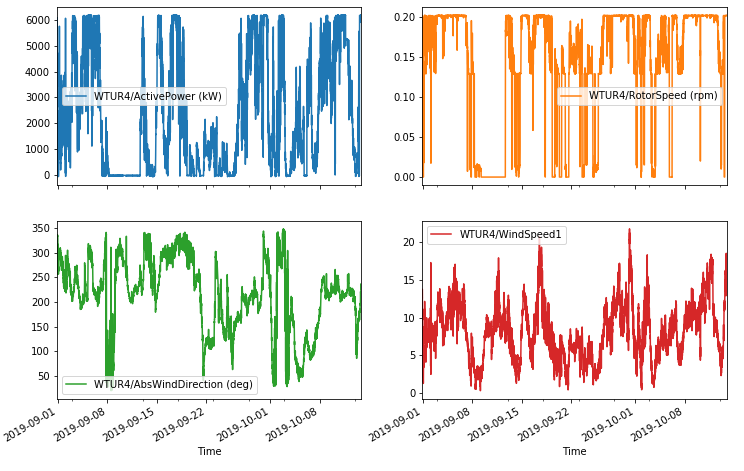
\includegraphics[width=0.6\textwidth]{data_exp/one_turbine_all_vals}
    \end{center}
    \caption{The data from one wind turbine} 
    \label{fig:data_one_wt}
\end{figure}

\section{Explained Varience of Principal Components}

One interesting point of comparison for the different wind turbines is the cumulative explained variance of a wind turbine for a given set of principal components. 
The total variance is the sum of the variences of the individual principal components. 
Since these multivariate time series have four dimensions four principle components should then be able to explain the variance of the entire dataset, as they are the eigenvectors of the covarience matrix of the time series. 
The explained variance of a principal component is the ration of the variance of said component to the total variance, and the cumulative explained variance of $n$ principal components is the sum of the explained variance of the $n$ first principal components. Since these turbines are in the same wind farm they are exposed to roughly the same environmental conditions, and one would expect them to have similar cumulative explained variance curves.

\begin{figure}[h]
    \begin{center}
    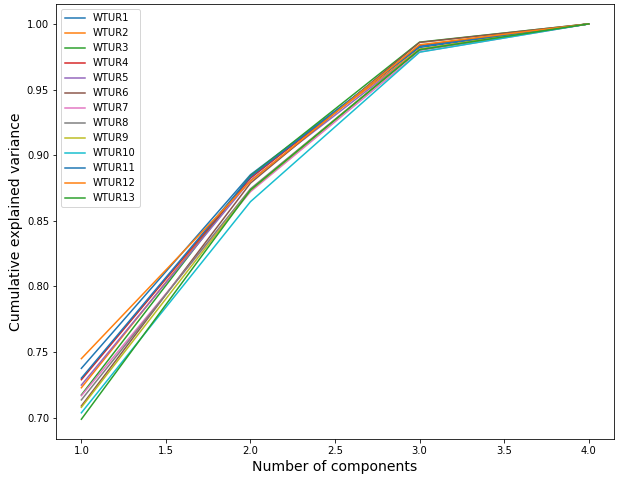
\includegraphics[width=0.5\textwidth]{data_exp/cumulative_explained_variance}
    \end{center}
    \caption{Cumulative explained variance for a given number of principal components} 
    \label{fig:cum_exp_var}
\end{figure}

In figure \ref{fig:cum_exp_var} there is a plot of the cumulative explained varience of the 13 turbines for a given set of principal components. 
As expected the total variance can be explained by four principle components for all wind turbines. 
However, as the number of principal components decreases there is a greater variety in the cumulutive explained variance for the different wind turbines. 
For only one principal component the biggest difference in cumulative explained varience is between turbine two at 75$\%$ explained variance, and turbine 13 at 70$\%$ explained variance.
This difference is not that substantial, from the plot in figure \ref{fig:cum_exp_var} one can see that all the curves follow more or less the same shape, so one cannot conclude that any of these curves are due to anomolous behaviour. \smallskip

\section{Reconstruction Error}

\begin{figure}[h]
    \begin{center}
    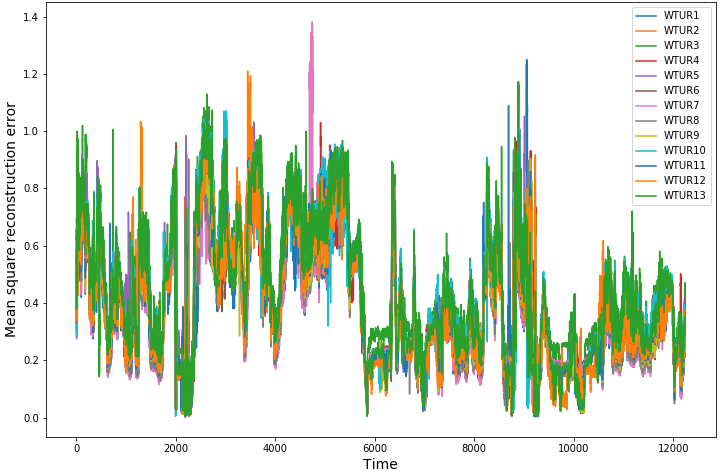
\includegraphics[width=0.5\textwidth]{data_exp/reconstruction_error}
    \end{center}
    \caption{Reconstruction error, when representing data with two principal components} 
    \label{fig:recon_error}
\end{figure}

Another indicator of anomolous behaviour is if the multivariate time series associated with a turbine has a significantly different $R_e$ compared to the multivariate time series of the other turbines in the wind farm. 
Figure \ref{fig:recon_error} shows the total MSE of the reconstructed time series associated with the different wind turbines. 
Here too, one can observe that the different wind turbines all follow approximately the same curve with regard to reconstruction error. 
With the exception of turbine seven has a slight spike at round about 5000 samples. 
To get a better reference of what constitutes anomolous behaviour, the data from one turbine will be artificially perturbed in the coming section. 

\section{Artificially Perturbation of Data}

\begin{figure}
    \begin{center}
    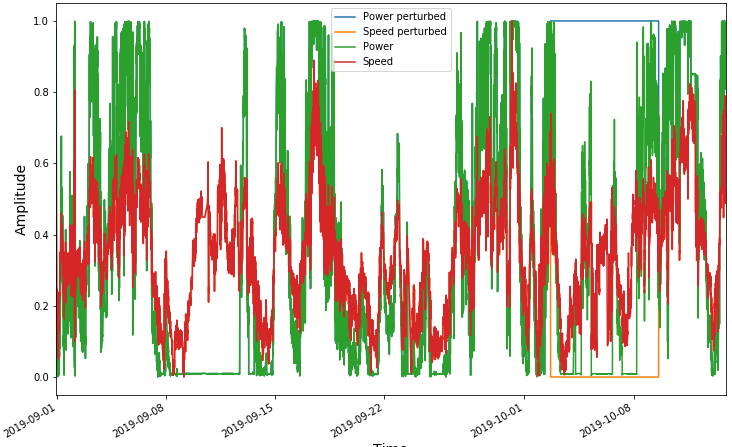
\includegraphics[width=0.5\textwidth]{data_exp/perturbed_vs_unperturbed}
    \end{center}
    \caption{Illustration of the perturbed data} 
    \label{fig:illu_perturbed_data}
\end{figure}

To artificially perturb the data 2000 samples from turbine 12 are changed. 
Sample 9000 to sample 1100 of the wind-speed and power time series are set to one and zero respectively.
Figure \ref{fig:illu_perturbed_data} illustrates this. 
This drastically changes the curve of cumulutive explained variance which is depicted in figure \ref{fig:cum_exp_var_pert}, and the reconstruction error of the time series associated with turbine 12 which is depicted in figure \ref{fig:recon_error_pert_vs_unpert} and \ref{fig:recon_error_pert}.
From figure \ref{fig:cum_exp_var_pert} one can see that the cumulative explained variance curve of turbine 12 is significantly lower than the curves of the other turbines in the farm, giving a reference of how some anomolous behaviour would show up in a cumulative explained variance curve. 
In figure \ref{fig:recon_error_pert_vs_unpert} one can see the reconstruction error of turbine 12 increases overall after the perturbation, and increases even more in the particular samples where the time series was altered. 
Finally, if one compares the reconstruction error of the perturbed data of wind turbine with the reconstruction error of the original data from the other turbines in figure \ref{fig:recon_error_pert}, one can see that the spike in turbine seven mentioned earlier is of the same magnitude as the spike in the reconstruction error of wind turbine 12 when artificially perturbed. 

\begin{figure}
    \begin{center}
    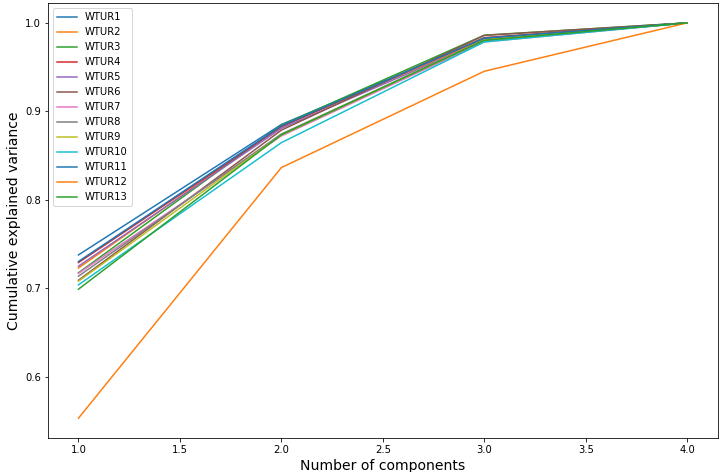
\includegraphics[width=0.5\textwidth]{data_exp/explained_variance_perturbed}
    \end{center}
    \caption{Cumulative explained variance for a given number of principal components with perturbed data} 
    \label{fig:cum_exp_var_pert}
\end{figure}

\begin{figure}
    \begin{center}
    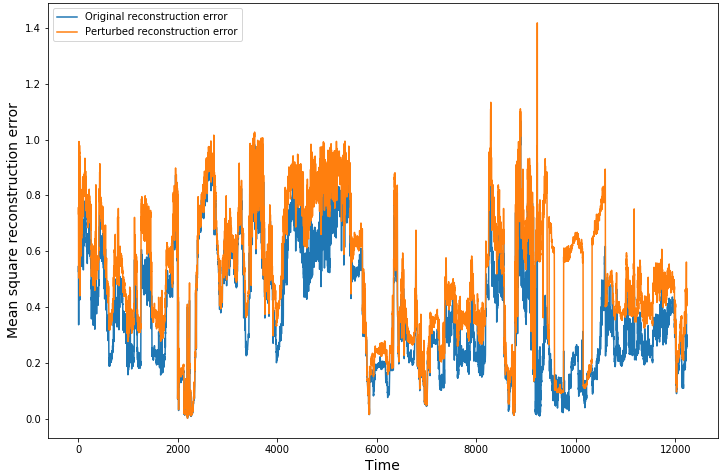
\includegraphics[width=0.5\textwidth]{data_exp/pert_vs_unpert_reconstruction_error}
    \end{center}
    \caption{Reconstruction of wind turbine 12 using two principal components, with original and perturbed data} 
    \label{fig:recon_error_pert_vs_unpert}
\end{figure}

\begin{figure}
    \begin{center}
    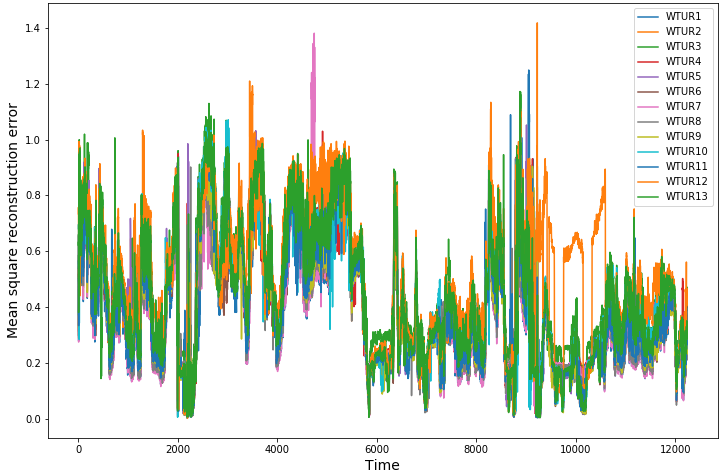
\includegraphics[width=0.5\textwidth]{data_exp/reconstruction_error_perturbed}
    \end{center}
    \caption{Reconstruction error, when representing data with two principal components using perturbed data} 
    \label{fig:recon_error_pert}
\end{figure}
\newpage
\chapter{Discussion} 

Machine learning methods used for wind turbine condition monitoring encountered in literature were divided into three categories: regression based models, supervised classification based models and unsupervised classification based models. 
The regression based models all had in common that they used some machine learning model to forecast the value of one sensor, or reconstruct their inputs, and then use the estimation error, or reconstruction error to indicate whether the wind turbine was operating outside its normal condition.
The supervised classification based models had in common that they trained supervised machine learning models directly to detect faults in the wind turbine based on the input of condition monitoring sensors, or images. 
The unsupervised classification models had in common that they used trained unsupervised machine learning models to detect anomalous behaviour in the wind turbines. 
A variety of machine learning models were applied, and a summary of their advantages and disadvantages can be found in table \ref{tab:ml_wt_sum}. \bigskip

The supervised classification models where disgarded because they all required labelled datasets with faults, which will not be available for a master thesis. 
The regression based models where also disgarded because they relied on complex machine learning models that would become too difficult to interpret, without labelled data. 
One of the four unsupervised classification methods stood out as applicable to the dataset that would be available for the master thesis. \textcite{fault_detect_PARAFAC_k_means} used a generalization of PCA to reduce the dimensionality of the multivariate time series produced by the wind turbines, and then used K-means clustering to cluster the wind turbines after dimensionality reduction. They acheived some accuracy with their model, but it remains untested for variable wind conditions. 

The literature revealed many approaches for feature-based and model-based representations of time series. 
Of the feature-based approaches PCA stood out as the most viable option for dimensionality reduction of time series. 
In chapter \ref{chap:data_exp} it is explored what the cumulative explained variance curve of the principal components, and reconstruction error can say about anomalous behaviour of single wind turbines in a wind farm. 
When the data of one wind turbine was artificially perturbed, it was evident in the cumulative explained variance curves. 
SAX was also found to be relevant for time series length compression. 
Of the model based approaches the ARMA model was used quite often in literature. Since ARMA models already are used to some extent for feature extraction of wind turbines monetoring systems explored in chapter \ref{chap:wt_monitoring}, it is considered very relevant as an option for model-based representation. 
HMM were also found to be viable options for model-based representation methods.
Probabilistic clustering systems that represented cluster centers with mixture models, and then clustered time series using expectation-maximization were found to be too computationally complex consider for the master thesis. 
Most of the clustering algorithms explored have open source implementations in python, and were considered worth testing with the exception of SOMs which would require careful design, and time consuming training, so they are not regarded useful for testing in a master thesis. 

\chapter{Conclusion and Future Work}
The objectives of this literature review have been to: Get an overview of the different machine learning methods used for monitoring of wind turbines, get an overview of the different feature-based, and model-based TSC methods and determine which of TSC techniques would be applicable for the clustering of time series produced by wind turbines. 351 articles were screened, and 96 articles were included in the review to fulfill the objectives. An overview of machine learning methods used for monitoring of wind turbines was given, and so was an overview of feature-based, and model-based TSC methods. 

For the master thesis the primary objective should be to test a model-based approach, and a feature-based approach. 
Based on the findings in the literature and the results of chapte \ref{chap:data_exp} the feature-based approach chosen is to reduce the dimensionality of the time series using PCA, and then clustering the feature-reduced time series. 
Similar to what has been done by \textcite{fault_detect_PARAFAC_k_means}. 
If this goes well one could consider trying out the approach of \textcite{multivariate_tsc_common_pca}: Use principal components to represent cluster centers, and reconstruction error to measure similarity.
The model-based approach should be to represent the time series with ARMA models, and cluster them with regard to their model parameters. Primarily one should try to represent univariate time series with ARMA models, but if there is time one could also represent multivariate time series with a vector AR model as done by \textcite{var_multivar_tsc}.

The second objective, if there is time would be to explore the use of HMMs to represent the time series, and clustering them with regard to their model parameters. The use of SAX to compress the length of the time series seems interesting, but does not promising enough to be prioritized over the other approaches. 


\section{Machine learning for wind turbine condition monitoring}

\begin{longtable}{p{0.03\textwidth}p{0.2\textwidth}p{0.3\textwidth}p{0.4\textwidth}}
    \hline
    Ref. & Input & Feature extraction method & Machine learning model \\
    \hline \hline
    \cite{ml_cm_wt_blade_ARMA_2018} & Vibration signal. & ARMA model and J48 decision tree & Tests a set of (38) meta-, misc-, rule- and tree-based classifiers for fault detection in blades. \\  \hline
    \cite{AD_and_fault_analysis_wt_DAE} & SCADA data. & & Deep auto-encoder made of Restricted Boltzman Machines (RBMs) to model normal behaviour of SCADA variables (gearbox and generator temperature). Uses $E_e$ for anomaly detection, with adaptive threshold set using extreme function theory (EFT). \\ \hline
    \cite{unsup_graphical_modeling_wt_cm} & SCADA data. & Spatiotemporal pattern network & Unsupervised use of RBMs for anomaly detection. \\ \hline
    \cite{fault_detection_and_isolation_using_classifier_fusion} & SCADA data. & Time-frequency domain analysis, DWT and ARMA model & Uses fusion of several classifiers for fault detection in a wind turbine.  \\ \hline
    \cite{lin_and_non_lin_feat_for_ice_detection_on_blades} & Ultrasonic testing. & Tests linear and non-linear PCA and ARMA models & Neighbourhood component analysis for feature selection. Tests 20 different supervised classifiers for detecting ice on blades. \\ \hline
    \cite{perf_mon_of_wt_using_extreme_func_theory} & Wind-Power curve. &  & Uses Gaussian Process regression with EFT to determine whether a particular power curve is an outlier.\\ \hline
    \cite{blade_damage_detection_sup_ml_alg} & Acustic emission. & FFT. & Uses Distinguishability Measure for feature selection, and logistic regression and SVC for binary blade fault classification. \\ \hline
    \cite{wt_cm_using_cloud_computing_and_HELM} & Power signal, wind speed and ambient temperature. & & Hierarchical Extreme Learning Machine (H-ELM) for detection of anomolous behaviour. \\ \hline
    \cite{GP_operational_curve_monitoring} & SCADA data. & & Gaussian processes regression to estimate wind-power curve \\ \hline
    \cite{high_freq_scada_perf_monit_sensitivity} & SCADA data. & & Tests KNN, random forest, and SVR to estimate power curve. Detects anomalies by $E_e$. \\ \hline
    \cite{dict_learning_monitor_wt_drivetrain_bearing} & Vibration signals. & & Uses unsupervised dictionary learning extracting features which are then used to determine fault in drivetrain bearings. \\ \hline
    \cite{ANN_damage_detection_gearbox_wt} & Oil temperature, wind speed, rotor speed and active power. & & Trains ANN to estimate vibration signal, uses $E_e$ for anomaly detection. \\ \hline
    \cite{multiway_PCA_multivar_inference_cm_wt} & SCADA data. & PCA. & Sets up baseline model using multiway PCA, then finds outliers by hypothesis testing whether multivariate distribution is equal to baseline. \\ \hline
    \cite{image_texture_analysis_FD_wt} & FAST wind turbine simulator. & Image texture analysis tools. & KNN, Linear Discriminant Model, decision trees, bag-tree, linear SVC.\\ \hline
    \cite{auto_associative_nn_wt_fault_detection} & SCADA data. & K-means for outlier elimination. & Uses Auto-Associative Neural Networks as an auto-encoder, and the Hotel T2 statistic as a dynamic threshold for the $R_e$.\\ \hline
    \cite{abnormal_detection_scada_data_mining} & SCADA data. & Grey correlation algorithm for eigenvector extraction. & Use genetic algorithm for feature selection, and SVR for estimating performance curves (active power, rotor speed and blade pitch angle). \\ \hline
    \cite{health_cond_model_nn_proportional_hazard_models} & SCADA data. & & Uses three NN for normal behaviour modelling of rotor speed, gearbox temperature and generator temperature. $E_e$ sendt to proportional hazard model which sets dynamic threshold. \\ \hline
    \cite{ice_detection_using_ITL} & SCADA data. & & Uses Inductive Transfer Learning and five differen ML classifiers for ice detection on blades. \\ \hline
    \cite{VMD_MPE_COVAL_fault_detection_gearbox} & Vibration signals. & Variational mode decomposition (VMD). & Uses multi-scale permutation entropy (MPE) used for feature selection, COVAL for domain normalization and an SVC for binary fault classification.\\ \hline
    \cite{SVR_blade_pitch_curve_cm} & SCADA data. & & Uses bins and SVR to estimate blade angle pitch curve. \\ \hline
    \cite{detecting_malfunctions_wt_generator_bearings_generic_vs_specific_models} & SCADA data. &  & Tests different architectures of ANNs to for estimating temperature of non-drive end bearing. Uses $E_e$ for anomaly detection. \\ \hline
    \cite{image_based_surface_damage_detection_DL_drone_inspection} & Images taken by drones & & Recurrent Convolutional Neural Network to classify structural damage in blades.\\ \hline
    \cite{image_based_YOLO_YSODA} & Uses images taken from ground level & & Convolutional Neural Network, and YOLO-based small object detection approach (YSODA) for damage detection in blades and hub.\\ \hline
    \cite{vibration_acustic_decision_tree_SVM_gearbox} & Vibration signals, acustic emission and oil particle analysis & DWT. & Uses decision tree for feature selection, and SVC for assessing fault severity in gearbox\\ \hline
    \cite{AI_image_analytics_2_classify_blade_defects} & Uses images taken from ground level & & Convolutional Neural Network to detect cracks $\&$ damage in blades.\\ \hline
    \cite{dirt_n_mud_detection_using_guided_waves} & Ultrasonic testing & PCA and ARMA models. & Neighbourhood Component analysis for feature selection and an ensamble of KNN, linear SVC, decision trees, LDA and subspace discriminant to estimate amount of dirt and mud on blades. \\ \hline
    \cite{fault_classification_using_CSO_SVM} & Uses pitch position, rotor speed and generator speed. & & Detects faults with an SVC with parameters optimized by Cuckoo-swarm optimization. \\ \hline
    \cite{vibration_ARMA_decision_tree_cm_wt} & Vibration signals & ARMA model. & Dominating features selected with J48 decision tree, fault classification done with Bayesian- and lazy classifiers. \\ \hline
    \cite{integrated_cm_bearing_fault_wt_gearbox} & Vibration signals, acustic emission and oil particle analysis & DWT and PCA. & Dominating features selected with decision tree, fault detection done with SVC. \\ \hline
    \cite{blade_defect_detection_imaging_array} & Images taken from imaging array & & Uses a deep neural network for binary classification of blade defects. \\ \hline
    \cite{unsupervised_AD_blade_damage_deep_features_images} & Uses images taken by drone & Uses a CNN trained on an unrelated image dataset to extract general features. & Compress features with PCA, and pass them to a unsupervised one-class SVM. \\ \hline
    \cite{RF_XGB_fault_detection} & Uses the FAST wind turbine simulator to get SCADA data. & Random forest. & Uses XGBoost to train an ensamble of classifiers for specific faults. \\ \hline
    \cite{CBPM_ABPM_maintainance_model} & SCADA data. & & Uses several ANN to build a normal behaviour model of temperature in gearbox and high speed shaft, then uses $E_e$ together with the age of the age of the turbine to predict anomolous behaviour.\\ \hline
    \cite{improved_power_curve_monitoring_of_wt} & SCADA data. & & Uses Pearson product-moment rank correlation to select features, and applies different ANN structures to predict the active power. \\ \hline
    \cite{DBN_simulink_SCADA_FD} & SCADA data from a simulink model of a wind turbine. & & Uses DBN for detecting anomolous behaviour. First traines individual RBMs to recreate input, and then uses labeled data to fine tune DBN to detect faults. \\ \hline
    \cite{wt_gearbox_bearing_temp_KS_CNN} & SCADA data. &  & Uses kolmogorov-smirnov test to compare different turbines at same moment in time combined with the $E_e$ of the gearbox bearing temperature of an ANN to detect anomalies.\\ \hline
    \cite{fault_monitoring_HMM} & Vibration signals. & Approximates vibration distributions at different rotor speeds with Weibull distribution. & Uses a HMM for statistical fault detection. \\ \hline
    \cite{model_based_fuzzy_logic_cm_wt} & SCADA data. & & Compares linear models, ANNs and state-dependent parameter models for fault detection. \\ \hline
    \cite{fault_detect_PARAFAC_k_means} & SCADA data. & parallel factor analysis (PARAFAC) as a decomposition method & uses K-means clustering after decomposition for fault detection. \\ \hline
    \cite{online_fd_using_PCA_different_operating_zones} & Uses a wind turbine simulator for SCADA data. & & Multiple PCA models are as a statistical reference reflecting the data variability in local zones and used in parallel for online fault detection. \\ \hline
    \cite{roller_bearings_cm_fisher_score_and_permutation_entropy} & Vibration signals. & Variational mode decomposition & Uses Fisher score and ReliefF algorithm for feature selection. Feeds selected signals into a multi-class SVC for bearing fault detection. \\ \hline
    \cite{deep_learning_for_imbalanced_class_detection_bearing_cm} & SCADA data. & & Uses deep neural networks for detection of icing on the blades. \\ \hline
    \cite{reliability_analysis_detecting_FA_NN_wt} & SCADA data. & & Combines NN with alarms generated by SCADA system to reduce false alarm rate. \\ \hline
    \cite{DBN_chicken_swarm_optim} & SCADA data. & & Uses K-means clustering to partition turbines into different operating states, and a specific DBN of RBMs for each cluster to forecast the gearbox main bearing temperature. Uses $E_e$ to detect anomalies, threshold set by Mahalanobis distance. \\ \hline
    \cite{vibration_fault_diagnosis_wt_planetary_gearbox} & & & This is a literary review of vibration based condition monitoring and fault diagnosis of planetary gearboxes in wind turbines. \\ \hline
    \cite{ml_for_wt_cond_monit_rev} & & & This is a literary review of machine learning methods used for condition monitoring of wind turbines. \\ \hline
    \hline
    \caption{Summary of machine learning methods for wind turbine condition monitoring}
    \label{tab:machine_learning_wt_cm_summary}
\end{longtable}
\section{Time-Series Clustering}

\begin{longtable}{p{0.03\textwidth}p{0.17\textwidth}p{0.25\textwidth}p{0.25\textwidth}p{0.2\textwidth}}
    \hline
    Ref. & Representation & Similarity measure & Clustering Algorithms & Evaluation \\
    \hline 
    \hline
    \cite{mixture_gaussian_hmm} 		    & Mixture Gaussian hidden Markov model (MGHMM).& & Expectation-maximization (EM).& Bayesian information criterion (BIC).\\ \hline
    \cite{financial_tsc_variance_ratio}	    & Variance ratio statistics.& Euclidean distance.& Hierarchical clustering mainly, and K-means.& Duda-Hart $Je(2)/Je(1)$ indices.\\ \hline
    \cite{hmm_pm10_quantifying_impacts}     & HMM. States correspond to concentration regimes.& Which state each HMM is in.& Cluster together TS with corresponding HMMs in the same state.& \\ \hline
    \cite{tsc_rev}                          & This is a review of time series clustering.& & & \\ \hline
    \cite{ghsom_optimal_hedge_ratio}        & Raw TS and some extracted statistics: variance, covariance, spread and differences.& & Growing hierarchical self-organizing map (GHSOM).& \\ \hline
    \cite{hier_clust_w_state_space_models}  & Linear combinations of spline basis functions.& Euclidean distance.& State space modelling, K-means and complete-linkage hierarchical clustering.& L-curve and gap statistic.\\ \hline
    \cite{topology_for_shape_based_tsc}     & EMD for filtering out stochastic components, then extract topological features.& Euclidean distance.& K-means.& Precision, recall, F1-score and Matthews correlation coefficient.\\ \hline
    \cite{community_detection_networks_tsc} & Construct network between time series using dissimilarity matrix. Use KNN, and $\epsilon$-NN to create networks from matrix.& Test a multitude of different distance functions. DTW performs best.& Test many community detection algorithms to sort network into clusters.& Rand index.\\ \hline
    \cite{clust_large_datasets_aghabozorg}  & Symbolic Aggregate ApproXimation (SAX).& Approximate distance (APXDIST), Euclidean distance, and DTW.& Custom three step algorithm (MTC), with preclustering, sub-clustering, and merging to form final clusters.& Accuracy, precision, recall and F-measure.\\ \hline
    \cite{garch_robust_tsc}                 & Generalized autoregressive conditional heteroskedasticity (GARCH) model.& Tests different metrics based on squared Euclidean distance between unconditional volitility and time varying volitility.& Tests different variations of fuzzy C-medoids. & Xie-Beni index, and Fuzzy Rand index.\\ \hline
    \cite{BSLEX_nonlin_nonstat_tsc}         & Bispectral Smoothed Localized Complex EXponential (BSLEX) algorithm.& Aggragated quasi-distance between smoothed bispectra across blocks.& Agglomorative hierarchical clustering with Ward's linkage.& Silhuette index as stopping criterion, and Rand Index, entropy and purity to evaluate cluster effectiveness.\\ \hline
    \cite{multivariate_tsc_hmm}             & HMMs.& Kulback-Leibler distance between the likelihood of observation sequency $T$ given HMM $\lambda$.& K-medoids.& Silhouette index, Bavies-Bouldin index and Dunn index.\\ \hline
    \cite{copula_fuzzy_tsc_spatial}         & Copula-based model for time series.& P-norm of difference between copula of two points, and upper bound copula.& Fuzzy C-medoids.& Fuzzy Silhouette (FS) index, adjusted Rand index (ARI), fuzzy Rand index (FRI).\\ \hline
    \cite{shape_feat_mod_tsc_rfa}           & DWT, SAX and AR model.& MINDIST, Euclidean, Minkowski, Pearson correlation coefficient and DTW distance. & Agglomerative Hierarchical clustering with Ward linkage.& Uses the clusters produced to perform regional frequency analysis, and then evaluates model using bias, RMSE, relative RMSE (RRMSE) and Nash criterion.\\ \hline
    \cite{ica_tsc_sea_level}                & Independent component analysis (ICA).& Not specified.& Hierarchical clustering with complete linkage.& \\ \hline
    \cite{apxdist_sax_k_modes}              & SAX.& APXDIST between symbolic representations of TS.& Extended version of K-modes.& SSE for stopping criteria, Rand index, Normalized Mutual Information (NMI), Purity, Jaccard, F-measure, Folks and Mallows (FM) and entropy.\\ \hline
    \cite{multivar_tsc_riemann_manifold}    & Tranforms the covariance matrices of the time series into a tangent space.& Euclidean distance.& Hierarchical clustering with average linkage.& \\ \hline
    \cite{tsc_total_variation_distance}     & Normalized spectral densities.& Total variation distence.& Agglomorative hierarchical clustering with complete and average linkage.& Dunn's index.\\ \hline
    \cite{temporal_tsc_threshold_ar_models} & Self-exciting threshold autoregressive model (SETAR).& Primarily tests Euclidean distance, Haussdorf distance and DTW, but, tests 22 different ones.& Primary method is spectral clustering, but also tests K-medoids, and fuzzy C-means.& Measures accuracy of method on clustering simulated data, and uses Gap statistic as stopping criterion.\\ \hline
    \cite{tsc_ar_metric_air_pollution}      & AR model.& A type of exponential Euclidean distance.& Fuzzy C-medoids.& Fuzzy Silhouette index.\\ \hline
    \cite{wavelet_multivar_tsc_multi_pca}   & Continous wavelet transform (CWT).& Multi-scale PCA similarity matric.& Fuzzy C-means.& Precision and recall of classification according to labels, and silhouette index.\\ \hline
    \cite{stock_price_tsc_regr_trees_som}   & Preprocessing using Hodrick-Prescott (HP) filter, feature extraction using state space models or regression trees.& & Self-organizing map (SOM).& Silhouette index as stopping criterion.\\ \hline
    \cite{ar_metric_trimmed_fuzzy_tsc_pm10} & ARIMA model.& Euclidean distance between AR weights.& Trimmed fuzzy C-medoids.& Decides number of clusters by looking at the rate of decrease, and second derivative of an objective function with regard to a trimming factor $\alpha$.\\ \hline
    \cite{dependency_tsc_energy_markets}    & Permutation based coding of time series.& Use four distance metrics based on mutual information, entropy and Cramer's V association measure.& Hierarchical clustering with single, complete and average linkage.& \\ \hline
    \cite{moar_mpl_tsc}                     & Mixture of autoregressions (MoAR) models.& & Maximum pseudolikelihood esitmation using EM algorithm. & \\ \hline
    \cite{copula_ica_tsc}                   & Use PCA and custom ICA algorithm for feature extraction.& Euclidean distance between extracted features.& Hierarchical clustering with average, single, complete and Ward linkage, and K-means.& CH, Friedman, C-index, Dunn's, SDbw and Silhouette index.\\ \hline
    \cite{tsc_slaughterhouse}               & Extracts various signal statistics, and performs feature extraction using R package ''Psych''.& Euclidean distance.& Hierarchical clustering with complete linkage.& \\ \hline
    \cite{ambient_air_vape_k_means}         & DWT with the Haar wavelet, and a globel sensitivity analysis.& Euclidean distance, to minimize variance.& K-means.& \\ \hline
    \cite{multivar_tsc_community_detection} & Multi-relational network in topological domain, static (time-invariant), and dynamic (time-varying).& & Multi-nonnegative matrix factorization. Compares their approach to three other community detection algorithms.& Rand index, adjusted Rand index and purity.\\ \hline
    \cite{fuzzy_c_means_pso_svd}            & Uses Singular value decomposition (SVD) to represent the cluster centroids.& Pearson correlation coefficient.& Fuzzy C-means with particle swarm optimization.& Precision, and F-measure.\\ \hline
    \cite{hysteresis_tsc_tensor_decomp}     & Multivariate time series are transformed into 3-order hysteresis tensors, then multilinear PCA is used to reduce dimensionality.& Tensor distance metric. Cluster centers initialized based on cycle feature variation.& Tensor K-means (CTKmeans).& RI, ARI, Jaccard coefficient and FM index.\\ \hline
    \cite{comp_many_model_based_tsc_GMM}    & Compares ten model-based clustering methods. GMM and Markov-switching model perform best.& & Expectation-maximization (EM). & Misclassification rates.\\ \hline
    \cite{dwt_hac_kmeans_som}               & Vari-segmented DWT.& Euclidean distance.& K-means, hierarchical agglomerative clustering and SOM.& \\ \hline
    \cite{xml_dft_delaunay_traingulation}   & Discrete Fourier transform (DFT).& Euclidean distance.& Delaunay Triangulation method.& Purity and F-measure.\\ \hline
    \cite{svd_birch_tsc_stock_price}        & Piecewise SVD, and piecewise aggregate approximation (PAA).& Euclidean Distance.& Balanced Iterative Reducing and Clustering using Hierarchies (BIRCH).& \\ \hline
    \cite{road_grade_china_pca_kmeans}      & Extracts signal statistics, and uses PCA for feature selection.& Euclidean distance.& K-means.& Analyses the correlations of specific features with different clusters.\\ \hline
    \cite{fragmented_periodogram}           & Fragmented periodogram.& Euclidean distance.& Spectral clustering.& \\ \hline
    \cite{auto_encoder_many_tsc_algorithms} & Extract statistical features of time series, then use a convolutional auto-encoder for further feature extraction.& Mainly Euclidean distance for the model-based approach.& K-means, hierarchical clustering with Ward linkage, spectral clustering, Gaussian mixture models, BIRCH, affinity propagation, mean shift, DBSCAN. &Adjusted Rand index. \\ \hline
    \cite{load_tsc_state_space_model}       & Compares a feature-based approach using PCA, with a model-based approach using state-space models for the individual time series.& Inverse exponential Euclidean distance for feature based approach, and Euclidean distance for model-based approach.& & Silhuette index as stopping criterion.\\ \hline
    \cite{struct_damage_ar_fuzzy_c_means}   & AR model.& Euclidean distance.& Fuzzy C-means.& \\ \hline
    \cite{fstar_hac_tsc}                    & Flexible space-time autoregressive (FSTAR) models.& Use Wald statistic to compare model parameters of univariate STAR models, and p-value as a similarity metric.& Hierarchical agglomorative clustering.& ARI.\\ \hline
    \cite{multivariate_tsc_common_pca}      & Common PCA (CPCA).& Cluster centroids represented by common projection axis of all TS in a specific cluster, then reconstruction error of time series using cluster centroid used as similarity metric.& Custom algorithm, similar to K-means.& Precision.\\ \hline
    \cite{tensor_multi_elastic_kernel_tsc}  & Map the time series to multiple high-dimensional tensors using multiple kernals.& Matrix $L^p$-norms.& Self-developed multi kernal clustering algorithm (MKC).& NMI and Rand Index (RI).\\ \hline
    \cite{var_multivar_tsc}                 & Vector autoregressive (VAR) models.& Euclidean distance.& Test two self-developed algorithms based on performing statistical test of whether TS come from same DGN. & Purity index.\\ \hline
    \hline
    \caption{Summary of model based time-series clustering methods}
    \label{tab:machine_learning_wt_cm_summary}
\end{longtable}


\section{Code}

\begin{listing}[h]
    \begin{minted}
    	[
    	frame=lines,
    	framesep=2mm,
    	baselinestretch=1.2,
    	fontsize=\footnotesize,
    	linenos
    	]
    	{Python}
    	import pandas as pd
    	import numpy as np
    	import matplotlib as mpl
    	import matplotlib.pyplot as plt
    	import seaborn as sns
    	import statsmodels.api as sm
    \end{minted}
    \label{lst:clean}
    \caption{Module fetching and data cleaning}
\end{listing}


\printbibliography

\end{document}
